In traditional neural networks, the topology is fixed. The number of hidden layers and the number of neurons in each hidden layer are given. This makes it very easy to see the difference between two networks, since the only differences are the weights.

The downside is, that the performance of these networks heavily depends on the chosen topology, which leads to the conclusion that many networks would perform better if one had chosen a different topology.

NEAT proposes a technique to evolve the topology over time which allows the network to be better structured for a specific task then a configuration with hyper parameters.

The main problem of such a network, called \emph{Topology and Weight Evolving
Artificial Neural Network}, or TWEANN for short, is the \emph{competing conventions problem} \cite{Stanley2002}.
It means that two networks may generate the same solution to a problem at different points in time, thus appearing to be two distinct topologies.\\
This makes the algorithm mark them as not compatible for a genetic crossover during the mating phase.

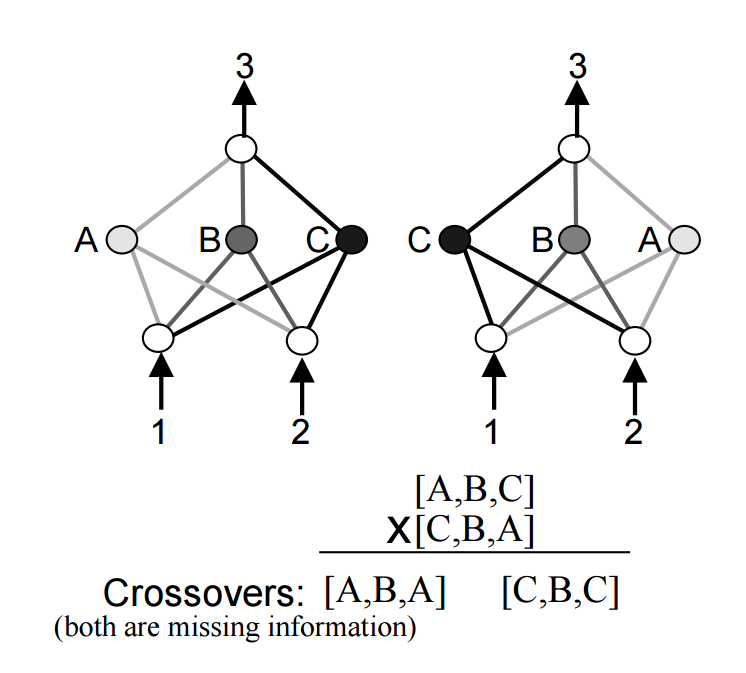
\includegraphics[scale=0.4]{competingconventions.png}

NEAT solves this problem by assigning each connection a \emph{historical marking}, which can be imagined as a serial number.\\
The first gene ever created is corresponds to a historical marking of one, the next one to two, and so on.\\
Every new gene is then first compared with all existing genes. If an identical match is found, the new gene gets the same historical marking as its twin. If not, the next biggest total number is assigned to it.

This way, during crossover, the algorithm doesn't have to check any complicated structural compatibility, but instead simply compares the historical markings of the two networks. If they are largely the same, the networks are suitable for a genetical exchange.
